\documentclass{beamer}
\usetheme{Madrid} % My favorite!
\setbeamercolor{normal text}{fg=purple}
\setbeamercolor{structure}{fg=blue} 
%\usetheme{Amsterdam} % My favorite!
%\usetheme{Boadilla} % Pretty neat, soft color.
%\usetheme{default}
%\usetheme{Warsaw}
%\usetheme{Bergen} % This template has nagivation on the left
%\usetheme{Frankfurt} % Similar to the default 
%with an extra region at the top.
%\usecolortheme{seahorse} % Simple and clean template
%\usetheme{Darmstadt} % not so good
% Uncomment the following line if you want %
% page numbers and using Warsaw theme%
%\setbeamertemplate{footline}[page number]
%\setbeamertemplate{}[frame number]
\setbeamercovered{transparent}
%\setbeamercovered{invisible}
% To remove the navigation symbols from 
% the bottom of slides%
%\setbeamertemplate{navigation symbols}{} 
%
\usepackage{array}
\usepackage{graphicx}
\usepackage{hyperref}
\usepackage{pxfonts}
\usepackage{listings}
%\usepackage{bm}         % For typesetting bold math (not \mathbold)
\logo{
\includegraphics[height=0.6cm]{logo.png}}
%
\title[foss.in | Hacking Android bootloaders]{Hacking Android bootloaders}
%\titlegraphic{
\includegraphics[width=3cm]{logo.png}}
\author{Sachin Patil}
%\logo{
\includegraphics[height=0.6cm]{logo.png}\vspace{210pt}}
%% 
\institute[IIT, Bombay]
{Indian Institute of Technology, Bombay \\
\medskip
isachin@iitb.ac.in
%{\emph{isachin@iitb.ac.in}}
}
%% \date{\today}
\date{November 29, 2012}
% \today will show current date. 
% Alternatively, you can specify a date.
%
\begin{document}

%% config for listing
\lstset{language=bash,
        numbers=left,
        numbersep=6pt,
        numberstyle=\tiny,
        showstringspaces=false,
        aboveskip=-50pt,
        frame=leftline,
        keywordstyle=\color{black},
        commentstyle=\color{blue},
        stringstyle=\color{black},
        }

%% 
%% slide 0
\begin{frame}
\titlepage
\end{frame}
%% 
%% slide 1
\begin{frame}
\frametitle{Why?}
\begin{block}                 
{why do I need it?}
\begin{itemize}
  \item I want dual/multiboot phone
  \item testing
  \item for fun
\end{itemize}
\end{block}
\end{frame}
%% 
%% slide 2
\begin{frame}
\frametitle{Introduction}
\begin{block}                 
{}
\begin{itemize}
  \item Two different versions of Android
    \begin{itemize}
      \item Ice cream sandwich - NAND
      \item Jelly bean - SDcard
    \end{itemize}
  \item Cyanogen(mod)
\end{itemize}
\end{block}
\begin{center}
  
\includegraphics[width=2cm, height=2cm]{cm.jpg}
\end{center}
\end{frame}
%% 
%% slide 3
\begin{frame}
\frametitle{Booting}
{Booting Android...}
\begin{center} 
  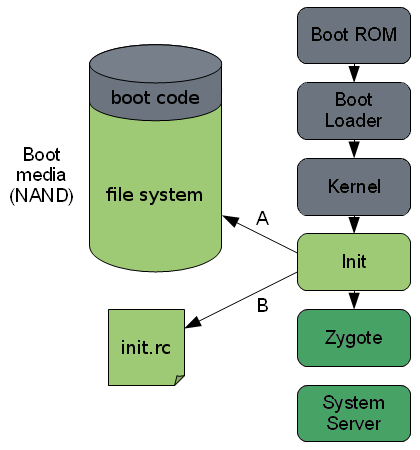
\includegraphics[width=6cm,height=6cm]{booting.png} 
\end{center} 
\end{frame}
%% 
%% slide 4
\begin{frame}
\frametitle{'/dev/mtd/' Partitions}
\begin{center}
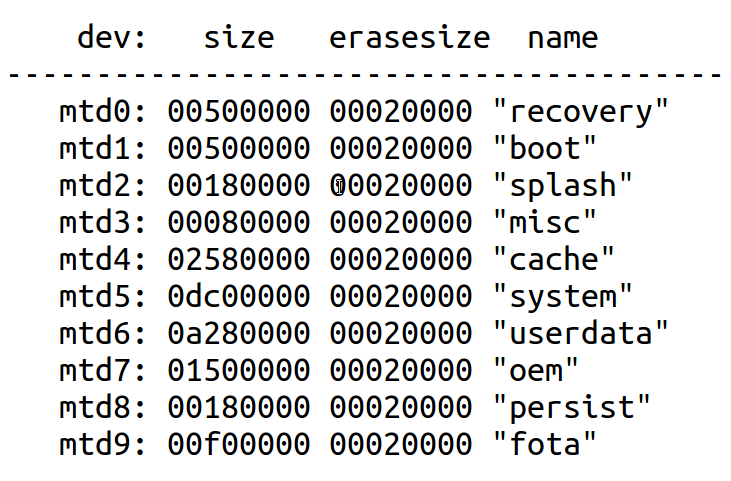
\includegraphics[width=7.5cm, height=5cm]{partition_idea_blade.png}
\end{center}
\end{frame}
%% 
%% slide 5
\begin{frame}
\frametitle{inside 'boot.img'}
\tt{tools/mkbootimg/bootimg.h}
\begin{center}
  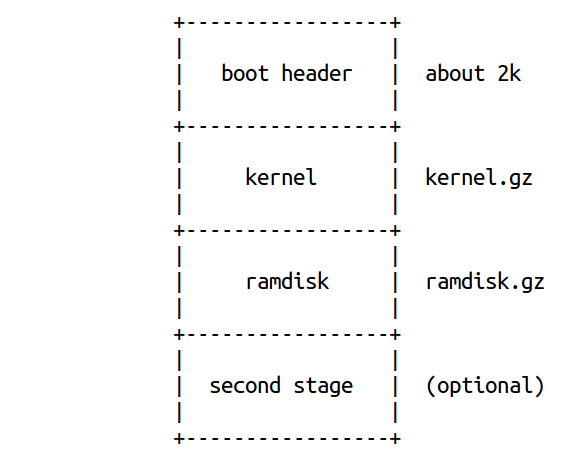
\includegraphics[width=6.5cm, height=5cm]{inside-bootimage.png}
\end{center}
\end{frame}
%% 
%% slide 6
\begin{frame}
\frametitle{Boot sequence}
\begin{center} 
  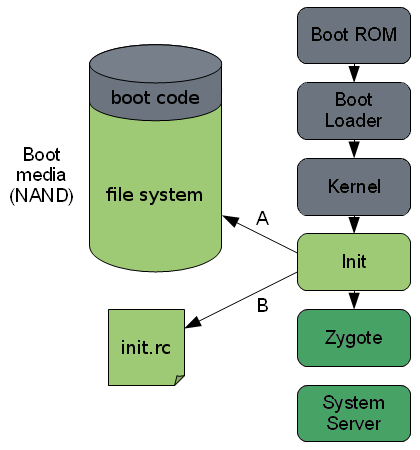
\includegraphics[width=6cm,height=6cm]{booting.png} 
\end{center} 
\end{frame}
%% 
%% slide 7
\begin{frame}
  \frametitle{init.rc}
  \begin{itemize}
  \item Mounting
  \item Setting premissions
  \item Starting services
  \end{itemize}
    \begin{center}
      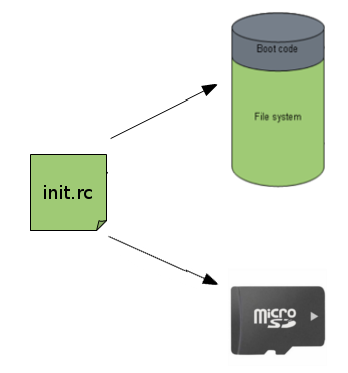
\includegraphics[width=5.5cm, height=5cm]{initrc.png}
    \end{center}
\end{frame}
%%
%% slide 8
\begin{frame}[fragile]
  \frametitle{\texttt{files}}
  \begin{semiverbatim}
    \pause
    \begin{lstlisting}
      `/META-INF/com/google/android/updater-script'
    \end{lstlisting}

    \pause
    \begin{lstlisting}[firstnumber=last]
      `boot.img/ramdisk/init.rc'
    \end{lstlisting}
  \end{semiverbatim}
\end{frame}
%% 
%% slide 9
\begin{frame}
\frametitle{\tt{init.rc}}
{}
\begin{block}
  {NAND}
  \begin{itemize}
  \item \tt{`mount yaffs2 mtd@system /system'} \\
  \item \tt{`mount yaffs2 mtd@system /system ro remount'} \\
  \item \tt{`mount yaffs2 mtd@userdata /data nosuid nodev'} \\
  \end{itemize}
\end{block}
\begin{block}
  {SDcard}
  \begin{itemize}
  \item \tt{`mount ext4 /dev/block/mmcblk0p3 /system'}
  \item \tt{`mount ext4 /dev/block/mmcblk0p3 /system ro remount'}
  \item \tt{`mount ext4 /dev/block/mmcblk0p2 /data nosuid nodev'}
  \end{itemize}
\end{block}
\end{frame}
%% 
%% slide 10
\begin{frame}
\frametitle{\tt {updater-script}}
\tt{`/META-INF/com/google/android/updater-script'}
\begin{block}
  {mount}
  \begin{itemize}
  \item \tt{mount("yaffs2", "MTD", "system", "/system");}
  \end{itemize}
  \center{\bf{to}}
  \begin{itemize}
  \item \tt{run\_program("/sbin/mount", "dev/block/mmcblk0p3", "/system");}
  \end{itemize}
\end{block}
\end{frame}
%% 
%% slide 11
\begin{frame}
\frametitle{\tt {updater-script}}
\tt{`/META-INF/com/google/android/updater-script'}
\begin{block}
  {format}
  \begin{itemize}
  \item \tt{`format("yaffs2", "MTD", "system", "0", "/system");'}
  \end{itemize}
  \center{\bf{to}}
  \begin{itemize}
  \item \tt{`run\_program("/sbin/mkfs.ext2", "dev/block/mmcblk0p3");'} 
  \end{itemize}
\end{block}
\end{frame}
%% 
%% slide 12
\begin{frame}[fragile]
  \frametitle{\texttt{/sdcard/bootnand.sh}}
  \begin{semiverbatim}
    \pause
    \begin{lstlisting}
      #!/bin/bash
      # boot from NAND 
    \end{lstlisting}

    \pause
    \begin{lstlisting}[firstnumber=last]
      # fill 'boot' partition with zero
      cat /dev/zero > /dev/mtd/mtd1
    \end{lstlisting}

    \pause
    \begin{lstlisting}[firstnumber=last]
      # flash image
      flash_image boot /sdcard/multiboot/boot.img
      echo "NAND boot enabled"
      reboot
    \end{lstlisting}

  \end{semiverbatim}
\end{frame}
%% 
%% slide 13
\begin{frame}[fragile]
  \frametitle{\texttt{/sdcard/bootsd.sh}}
  \begin{semiverbatim}
    \pause
    \begin{lstlisting}
      #!/bin/bash
      # boot from SDcard
    \end{lstlisting}

    \pause
    \begin{lstlisting}[firstnumber=last]
      # fill 'boot' partition with zero
      cat /dev/zero > /dev/mtd/mtd1
    \end{lstlisting}

    \pause
    \begin{lstlisting}[firstnumber=last]
      # flash image
      flash_image boot /sdcard/multiboot/bootsd.img
      echo "SDcard boot enabled"
      reboot
    \end{lstlisting}

  \end{semiverbatim}
\end{frame}
%% 
%% slide 14
\begin{frame}
\frametitle{\tt{terminal emulator}}
\begin{center} 
  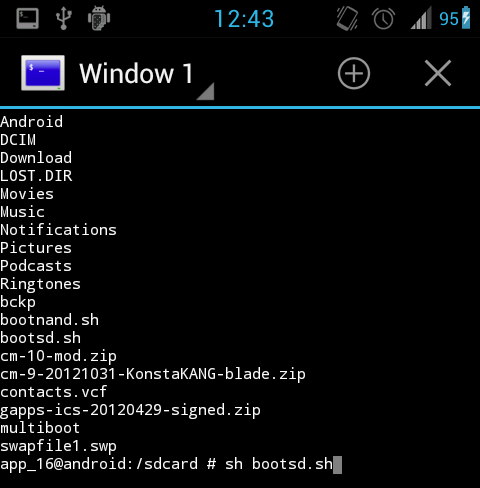
\includegraphics[width=6.5cm,height=7.5cm]{em2_cropd.png} 
\end{center} 
\end{frame}
%% 
%% slide 15
\begin{frame}{}
  \begin{block}{}
    \centerline{}
    \centerline{}
    \centerline{\href{file:///home/sachin/Videos/fossin/final.AVI}{Demo}}
    \centerline{}
    \centerline{}
  \end{block}
\end{frame}
%
% 
%% \begin{frame}{}
%%   \begin{figure}[ht]
%%     \includemovie[
%%       poster,
%%       text={\small (loading ...)},
%%       autoplay,
%%       mouse=true]
%%                  {8cm}
%%                  {6cm}
%%                  {/home/sachin/Videos/fossin/final.AVI}
%%   \end{figure}
%% \end{frame}
%
%
%% \begin{frame}
%% \frametitle{Summary}
%%   \begin{itemize}
%%   \item Booting sequence of Android
%%   \item modified \tt{`init.rc'} file from \tt{`boot.img'}
%%   \item modified \tt{`/META-INF/com/google/android/updater-script'}
%%   \end{itemize}
%% \end{frame}
%
%% \begin{frame}{Graphics} 
%% Here we include three images, one each of PDF, PNG, and JPG types. 
%% \begin{center} 
%%   
\includegraphics[width=0.3\textwidth]{logo.png} 
%% \end{center} 
%% \end{frame} 
%
%% \begin{frame}[fragile] % Notice the [fragile] option %
%% \frametitle{Verbatim}
%% \begin{block}
%% {block title}
%% \begin{itemize}
%%   \item itemized item 1
%%   \item itemized item 2
%%   \item itemized item 3
%% \end{itemize}
%% \end{block}
%% \end{frame}
% 
%% 
%% slide reference1
\begin{frame}{References}
  \begin{block}{web links}
    \scalebox{0.7}{%
      \vbox{%
        \begin{itemize}
        \item \url{elinux.org/Android_Booting}
        \item \url{android.googlesource.com/platform/system/core/+/master/init/readme.txt}
        \item \url{github.com/android/platform_system_core/blob/master/mkbootimg/bootimg.h}
        \item \url{http://www.youtube.com/watch?v=NIBrSyxSYLo}
        \end{itemize}
    }}  
  \end{block}

  \begin{block}{forums}
    \scalebox{0.7}{%
      \vbox{%
        \begin{itemize}
        \item \url{www.modaco.com/topic/356459-modtool-dual-boot-for-zte-blademodify-boot-tool-1408}  
        \item \url{forum.xda-developers.com/showthread.php?t=1823400}
        \end{itemize}
    }}  
  \end{block}
\end{frame}
%% 
%% slide reference2
\begin{frame}{References}
  \begin{block}{downloads}
    \scalebox{0.7}{%
      \vbox{%
        \begin{itemize}
        \item \url{https://github.com/psachin/Bootimg-scripts}
        \item \url{http://www.cyanogenmod.org/}
        \item \url{http://zteblade.eu/}
        \item \url{http://cyanogen-files.carneeki.net/flash_image.zip}
        \end{itemize}
    }}  
  \end{block}
\end{frame}
%% 
%% slide questions ???
\begin{frame}
\centerline{Questions?}
\end{frame}
%% End of slides
\end{document} 

